\section{Deep Learning Architectures \label{archi}}
We now turn our attention to the DL models that we have developed for help predict molecular properties.
\subsection{Overview}
    \begin{figure}[htbp]
        \centering
        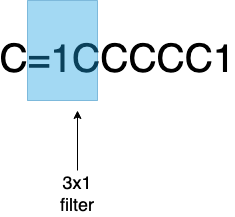
\includegraphics[width=0.15\textwidth]{figures/convonsmiles.png}
        \caption{A 3x1 filter in a 1-D Conv scanning a SMILES string. }
        \label{fig:conv-filter}
    \end{figure}
The main idea in our effort is to apply DL methods to the SMILE string to uncover patterns and crate models that predict molecular properties from first principles and without encoding rules from chemistry. Figure \ref{fig:conv-filter} show this idea in the context of a 1-D Convolutional Neural Networks (1-D Convs). In this figure, a $3 \times 1$ filter is used to scan the string and find patterns in the sequence of atoms and bonds. In practice, this filter does not run directly over the characters but instead  over the {\em character-level embeddings}  of the SMILES string. This approach will be explained in section \ref{embeddings}


In this paper, we shall focus on the use of 1-D Convs as the key methods used to build our models. Our work is still early, and we have also experimented with LSTM networks and Transformers. However,  1-D Convs have so far provided us with the best tradeoffs between training speed and prediction error. Comparing all these various methods in detail is part of our future work and is therefore outside the scope of this paper. 


    
Figure \ref{fig:ml-framework} shows the end-to-end machine learning framework that we propose. We start out with a sample of the data in PubChem that contains 600,000 examples. This data sets is split into standard training, validations and test sets. To train the models, the training data is fed as tensor input to the models. Next, a character-level embedding layer takes care of mapping the characters in the SMILE string into an $n$-dimensional vector space. These transformed data are then passed through several 1-D Conv layers to build and detect features in the SMILES strings. Later on, the tensors generated in these layers are ``flattened" from their multi-dimensional structures and fed into fully-connected layers, with the last layer producing the predictions of the model.
    \begin{figure}[htbp]
        \centering
        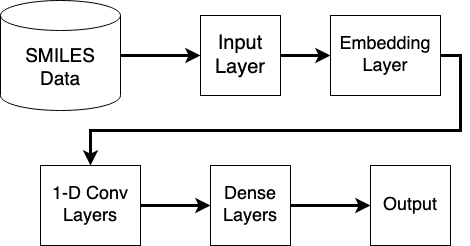
\includegraphics[width=0.4\textwidth]{figures/1DConvArch.png}
        \caption{Proposed end-to-end machine learning framework.}
        \label{fig:ml-framework}
    \end{figure}
\subsection{Character-level Embeddings \label{embeddings}}
DL expect their input as tensors, and the SMILES strings are not. Hence, we need a method to represent SMILES in tensor form. In the context of NLP, word embedding and character-level embedding have become the preferred way to accomplish, replacing one-hot encoding and bag-of-words models. The reason is that embeddings can retain the relationships, context, and meaning that existing between adjacent word or characters. 

In our efforts we do not word embeddings but rather character-level embeddings (REF). This is mainly because the structure of the SMILES does not maps with sentences separated by spaces as is the case for regular language sentences. Also, character level embeddings solve the {\em out-of-vocabulary words} issue, that often plagues word embedding methods.

  \begin{figure}[htbp]
        \centering
        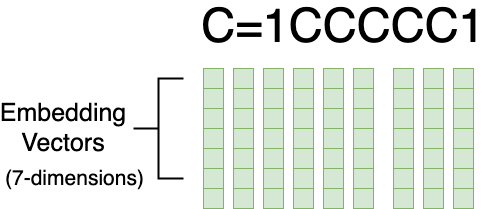
\includegraphics[width=0.4\textwidth]{figures/smileembedding.png}
        \caption{Embedding representation of a SMILES string.}
        \label{fig:smiles-to-embed}
    \end{figure}
Figure \ref{fig:smiles-to-embed} shows a SMILE string and a  character-level embedding into a 7-D vector space. Each character is mapped to a vector with 7 dimensions, and each component is a real number.  In practice, this vector space can have high dimensions, with some models using a dimension of 256. Finding the right dimension size is still much of an experimental issue. This SMILES  string in 
Figure \ref{fig:smiles-to-embed} can then be represented as  a $9 \times 7$ matrix, with each rows being a (transposed) embedding vector.
The standard practice is to thread the embedding as  another layer in the neural work, that can be trained to find the right values for the weights that produce the vectors. Some methods allow pre-training these weights on large corpus of target data set, and use transfer learning to enable researchers to focus on the design and tuning of the followup layers (i.e., the layers for the ``downstream task").

    % Model descriptions
    \subsection{Deep Learning to Predict Molecular Weight from SMILES}
        \begin{itemize}
            \item The first model we will discuss is a DL model that receives an embedded SMILES string as input and as a result returns its prediction of the molecular weight. This model is shown in Figure \ref{fig:mw-architecture}.
            \item Its architecture consisted first of a character embedding layer, that initially had random weights.
            \item This layer receives as input the pre-processed SMILES strings that had a length of 1000 and vocabulary size of 25.
            \item Its output is then passed to a 1D Convolutional Neural Network (CNN) that consists of 6 layers in total of 256 units each.
            \item The first two convolutional layers had a kernel of size 7x1 and were followed by 1D max pooling of size 3.
            \item The rest of the layers had kernels of size 3x1.
            \item The final layer was also followed by 1D max pooling layer of size 3.
            \item The result of the convolution was then passed to a flatten layer, which in turn is passed to the final three dense layers. 
            \item The first two dense layers consisted if 200 units and the final had only 1 unit. 
            \item All of the dense layers had a ReLU activation function.
            \item The final dense layer gives us the model's prediction of the molecular weight.
        \end{itemize}
    \subsection{Deep Learning to Predict XLogP from SMILES}
        \begin{itemize}
            \item The architecture for the second model is similar to the one used for predicting the molecular weight.
            \item The difference consists in the units and the kernel sizes used.
            \item This model it also receives as input SMILES strings of length 1000 and vocabulary size of 25.
            \item The embedding layer is once again followed by a CNN of 6 layers of 256 units each.
            \item The kernel sizes differ in this model the first 2 convolutional layers have a kernel size of 5x1 and the kernel size for the rest is 3x1.
            \item The 2 dense layers that follow now consist of 100 and 200 units respectively. 
            \item Finally, the final dense layer gives us the models prediction of the XLogP.
            \item The models architecture can be seen in Figure \ref{fig:xlogp-archi1}
        \end{itemize}
    \subsection{Deep Learning to Predict XLogP from SMILES and fragments}
        \begin{itemize}
            \item This model is similar to the first model, it differs in that it receives 2 inputs. 
            \item The model's architecture is shown in Figure \ref{fig:xlogp-archi2}
            \item Since for this model we have two sets of strings that we want it to use as input, we needed one embedding layer for each input received.
            \item One of the embedding layers receives the SMILES strings and the other receives the RECAP fragments of the chemical compound.
            \item These two embedding layers are then concatenated and supplied to the 1D CNN as input.
            \item The CNN and fully connected layers used had the same setup as the first model that predicted molecular weight.
            \item The output from the final dense layer is the predicted XLogP of the chemical compound.
        \end{itemize}
    
    % Figures
    \begin{figure}
        \centering
        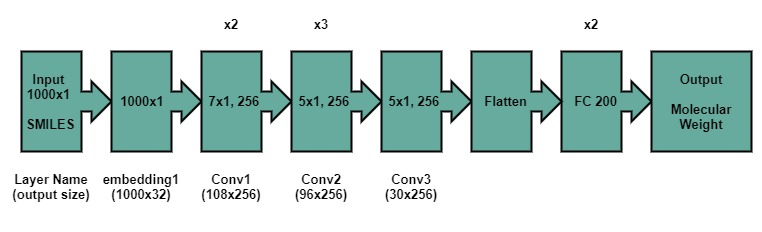
\includegraphics[width=0.5\textwidth]{figures/MW-model_arquitecture.jpg}
        \caption{The architecture of the model that predicts the molecular weight of a compound based on its SMILES string.}
        \label{fig:mw-architecture}
    \end{figure}
    \begin{figure}
        \centering
        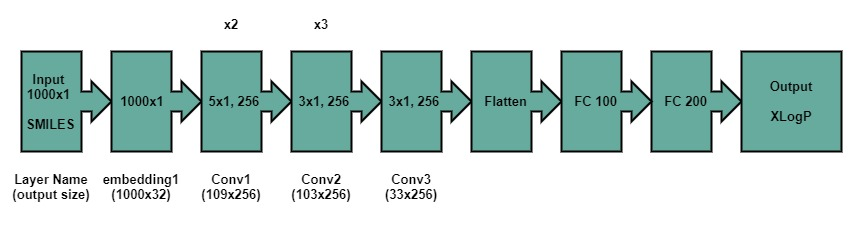
\includegraphics[width=0.5\textwidth]{figures/XLogP-model_arquitecture.jpg}
        \caption{The architecture of the model that predicts the XLogP of a compound based on its SMILES string.}
        \label{fig:xlogp-archi1}
    \end{figure}
    \begin{figure}
        \centering
        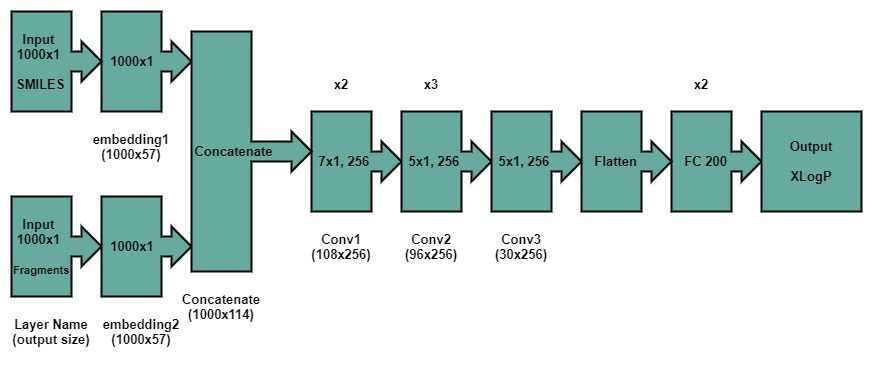
\includegraphics[width=0.5\textwidth]{figures/XLogP_frag_model_arquitecture.jpg}
        \caption{The architecture of the model that predicts the XLogP of a compound based on its SMILES string and RECAP fragments.}
        \label{fig:xlogp-archi2}
    \end{figure}